\section{Overall description}
\label{sect:overalldescription}

Here you can see how to include an image in your document.

\begin{sidewaysfigure}
\centering
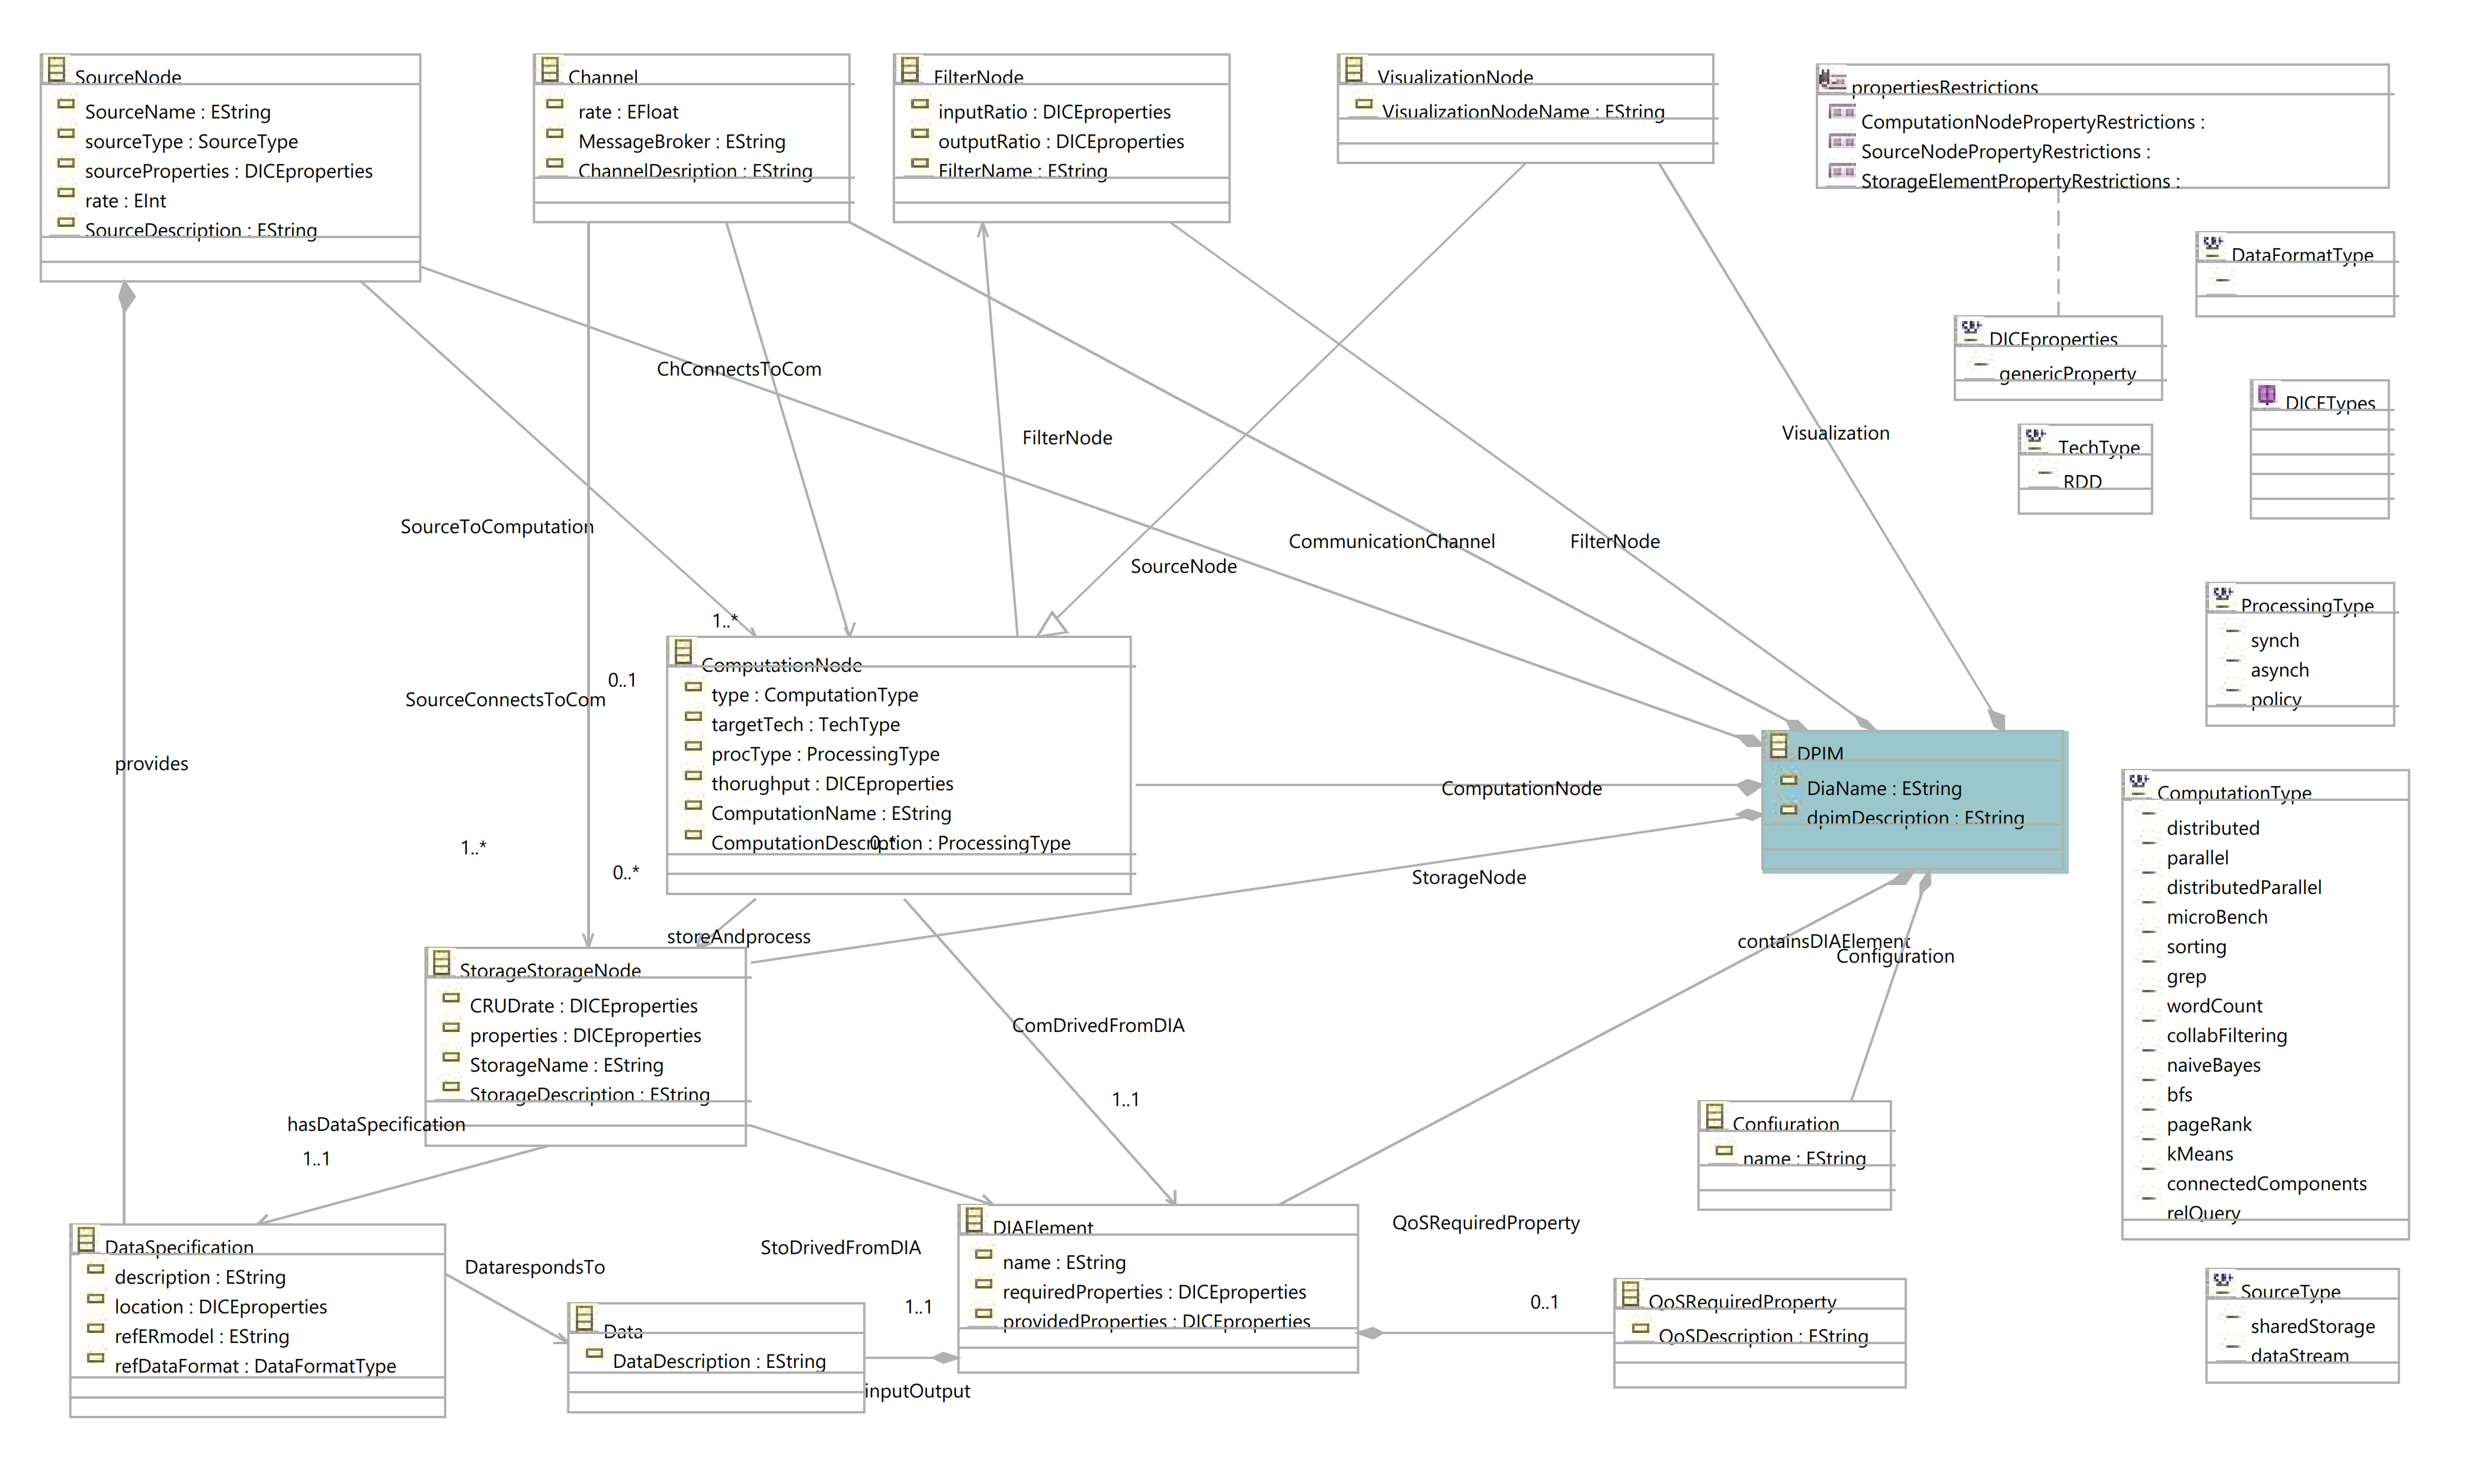
\includegraphics[width=\textwidth]{Images/11.png}
\caption{\label{fig:metamodel}DICE DPIM metamodel.}
\end{sidewaysfigure}

\begin{figure}
\centering
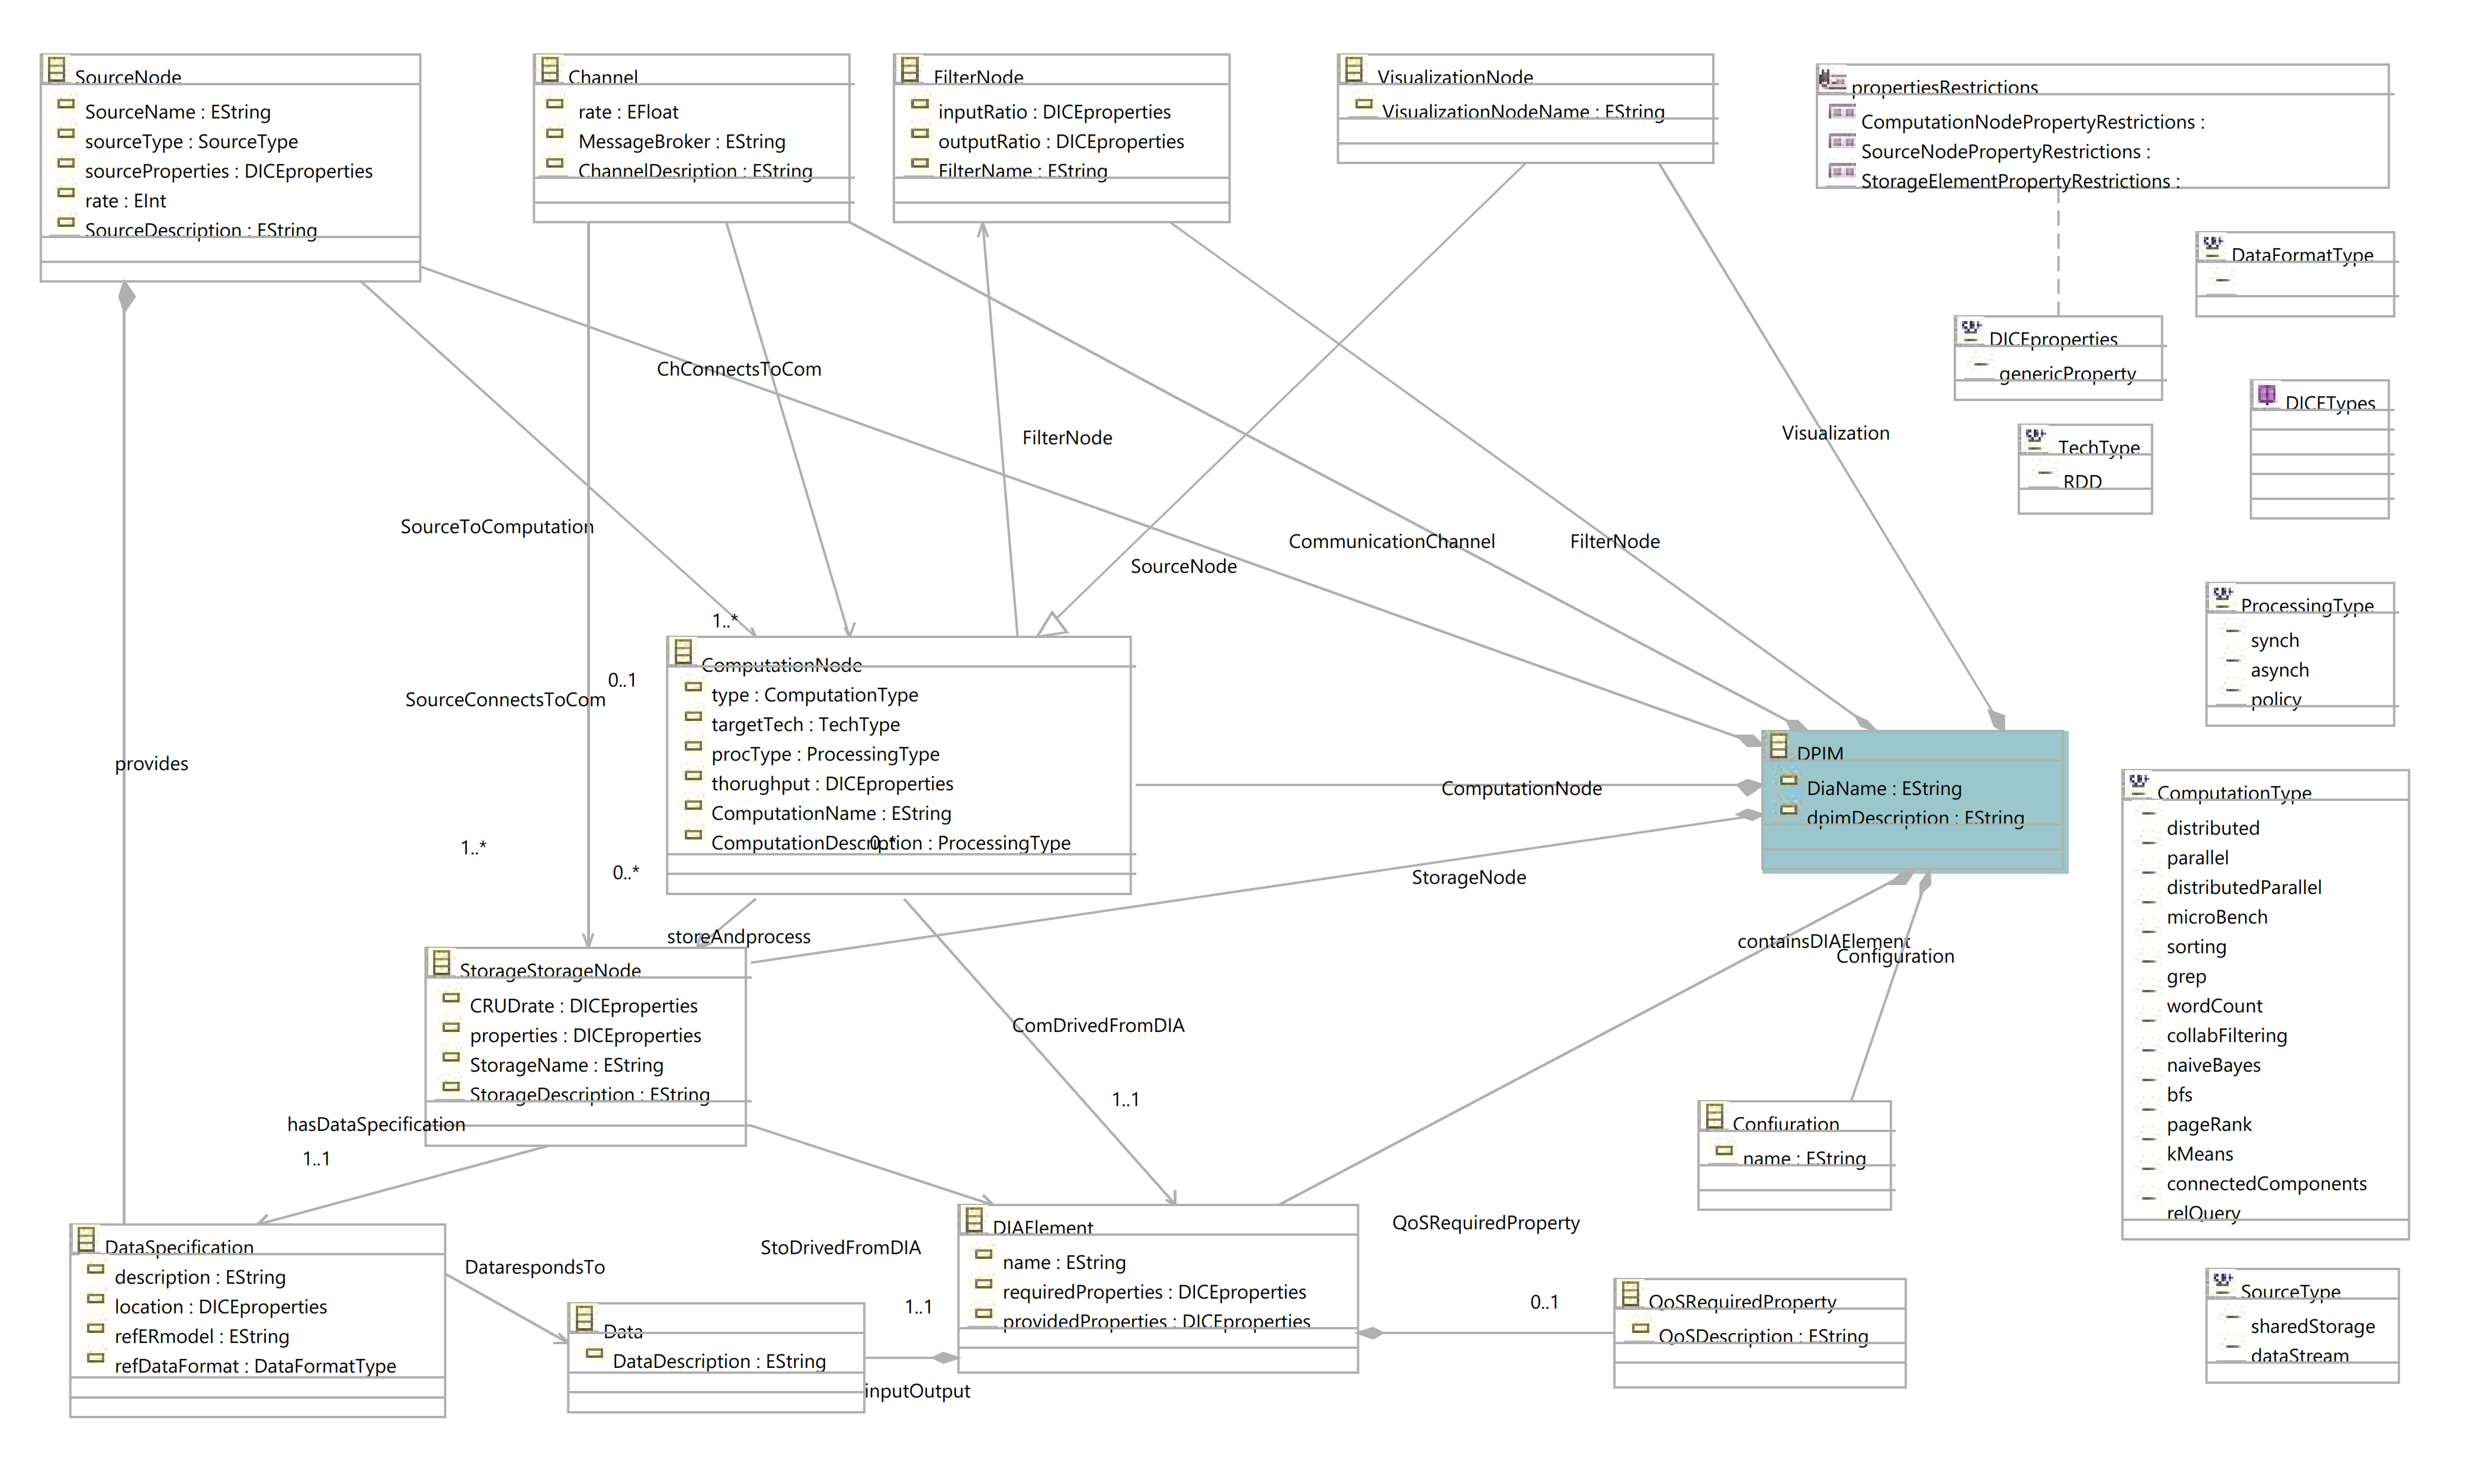
\includegraphics[width=\textwidth]{Images/11.png}
\caption{\label{fig:metamodel2}DICE DPIM metamodel in portrait form.}
\end{figure}

\subsection{Goals}
\label{sect:goals}

Shop Manager:
[G1] Allow a manager to sign on the system
[G2] Allow a manager to sign in the system
[G3] Allow a manager to register their store/stores on the system
    [G.3.1]Allow a manager to register basic info about the shop
	[G.3.2]Allow a manager to divide their store in areas 
	[G.3.3]Allow a manager to register the items in the areas 
[G4]Allow a manager to update the shop info
[G5]Allow a manager to check the general status of their shop

Customers:
[G6]Allow a customer to join the virtual queue from the spot*
[G7]Allow a customer to join the virtual queue from the app
[G8]Allow a user to sign on the system
[G9]Allow a registered-user to sign in the system
[G10]Allow a registered-user to book a shopping session at a grocery store
    [G9.2]Allow a registered-user to select the time and duration(between 		predefined options) for they session 	
    [G9.1]Allow a registered-user to select categories of items they are 	willing to 
    buy
[G11]Allow a registered-user to check retrieve informations about its previously booked visits
[G12]Allow a user to retrieve informations about the congestion of shops
[G12]Allow a customer to use a QR code to get access to the store 


* with the facility of a hardware support, it will be better specificed later on this document.

\subsection{Assumptions, dependencies and constraints}
\label{subsect:assumptionsdependenciescostraints}

\subsubsection{Domain Assumptions}
\label{subsubsect:domainassumptions}

Here we include domain assumptions.

Identify the relevant environment phenomena ("relevant" with respect to the goals). They are real world properties. They do not depend on the machine.

\subsubsection{Constraints}
\label{subsubsect:contraints}

Constraints: imposed by the client or the environment in which the system operates. 

Anything that will limit the developer’s options (e.g. regulations, reliability, criticality, hardware limitations, parallelism, etc.)


\subsection{Product perspective}
\label{subsect:productperspective}

Here we include scenarios and further details on the shared phenomena and a domain model (class diagrams and statecharts).

Describes external interfaces: system, user, hardware, software; also operations and site adaptation, and hardware constraints

\subsubsection{scenarios}
\label{subsubsect:scenarios}

“A narrative description of what people do and experience as they try to make use of computer systems and applications”.
A concrete, focused, informal description of a single feature of the system to be.

Heuristics for finding scenarios:
\begin{itemize}
    \item Which user groups are supported by the system to perform their work?
    \item What are the primary tasks that the system needs to perform?
    \item What data will the actor create, store, change, remove or add in the system?
    \item What external changes dows the system need to know about?
    \item What changes or events will the actor of the system need to be informed about?
\end{itemize}

\subsubsection{Use cases}
\label{subsubsect:usecases}

Here we generalize scenarios. Keep use cases small (no more than two/three pages).
Srtucture the description in terms of:
\begin{itemize}
    \item use case name: verb that indicate what the user is trying     to accomplish;
    \item participating actors;
    \item entry condition;
    \item flow of events: The steps accomplished by actors and those accomplished by the system should be clearly distinguished and the causal relationship between steps should be clear;
    \item exit condition;
    \item exceptions;
    \item special requirements (constraints, nonfunctional requirements).
\end{itemize}

\subsubsection{Class diagrams and statecharts}
\label{subsubsect:domainmodel}

What should we model? The objects and people that are of interest for the given problem. The relevant phenomena. The goals, requirements, and domain assumptions.

How do we find objects? Analyze any description of the problem, the application domain, the scenarios and use cases. 

to model dynamic behavior of a single object we use state machine diagram.

From the flow of events in the use case or scenario, proceed to the sequence diagram. A sequence diagram is a graphical description of objects participating in a use case or scenario using a DAG (directed acyclic graph) notation.

Consider using state diagrams and activity diagrams.

What is the structure of the world? $\rightarrow$ Create class siagrams for static information models (UML). Is there any state change in an object that is to be defined explicitly? $\rightarrow$ Create state diagrams for dynamic class behavior models. How is the expected interaction between the software to be and the environment? Create sequence diagrams from use cases for dynamic object behavior instance examples; or create activity diagrams when you want to highlight important process.

UML does not help us in expressing assertions, we can complement its usage with some formal or informal description of these assertions.

\subsection{Product functions}
\label{subsect:productfunctions}

Here we include the most important requirements.

\subsection{User characteristics}
\label{subsect:usercharacteristics}

Here we include anything that is relevant to clarify their needs.

\subsubsection{Actors}
\label{subsubsect:actors}

Customer: a person who grocery shops.
Unregistered user: a customer using CLup without being registered. They can join the virtual queue and ask/receive updates.
Registered user/User: a customer using Clup and who is registered on the system. They can join the virtual queue, book a shopping session and ask/receive updates.
Shop manager: a person who register their shop on Clup. A shop manager can register multiple shop on the system.
Shop: a grocery shop registered on the system. It updates periodically the people present in the store and sends updates to the manager.

\subsection{Phenomena [sezione provvisoria]}
\label{subsect:phenomena}

The machine: the portion of system to be developed.
The world (a.k.a. the environment): the portion of the real-world affected by the machine.
Requirements engineering is concerned with phenomena occurring in the world, as opposed to phenomena occurring inside the machine.

Goals are prescriptive assertions formulated in terms of \textbf{world} phenomena (not necessarily shared).
Domain properties/assumptions are descriptive assertions assumed to hold in the \textbf{world}.
Requirements are prescriptive assertions formulated in terms of \textbf{shared} phenomena.
Requirements are a bridge from the \textbf{machine} to the real \textbf{world}.

Find all the possible phenomena, for each one specify if its shared or not and who controls it (world or machine). 

All phenomena observed:

\begin{tabular}{|l|c|c|}
    \hline
    \textbf{Phenomenon} & \textbf{shared} & \textbf{controlled by}\\
    \hline
    User downloads the app & ? & ? \\
    Shop owner signs up to the app & ? & ? \\
    Customer signs up to the app & ? & ? \\
    Shop owner signs in & ? & ? \\
    Customer signs in & ? & ? \\
    Shop owner install a QR codes scanner & ? & ? \\
    \hline
    User wants to go to grocery store & ? & ? \\
    User searches a store in the CLup app & ? & ? \\
    User retrieve information about the queue of a shop & ? & ? \\
    User "lines up" for a store & ? & ? \\
    User searches information about his turn in the queue & ? & ? \\
    User receives notifications/updates about his position in the queue & ? & ? \\
    User receives a notification about special changes on the queue & ? & ? \\ %because of possible modifications from the manager, anche se non so se abbia senso sta cosa
    User goes to the grocery store & ? & ? \\
    USer enters the grocery store & ? & ? \\
    User shows his QR code to the store's scanner before going inside & ? & ? \\
    User does the shopping & ? & ? \\
    User shows his QR code to the store's scanner before going out & ? & ? \\
    User exits the grocery store & ? & ? \\
    
    %TODO:
    %Customers without CLup app reaches the store & ? & ? \\
    %Manager enqueue a customer & ? & ? \\
    %Manager checks esitmated queue time for customers he has put in queue & ? & ? \\
    %Manager communicates to CLup a customer has entered the store & ? & ? \\
    %Manager communicates to CLup an user ha exit the store & ? & ? \\
    
    User leaves the queue & ? & ? \\
    User doesn't show up & ? & ? \\
    User shows up early & ? & ? \\
    \hline
    User cheks available visits for a store & ? & ? \\
    User specifies the categories he is interested in & ? & ? \\
    User books a visit to the grocery store & ? & ? \\
    User checks his booked visits & ? & ? \\
    User receives notification/reminders about an imminent booked visit & ? & ? \\
    User receives notification about special changes on the visit & ? & ? \\
    Booked user is added to the queue & ? & ? \\ %idea per come implementarlo: una persona fa una prenotazione, il programma automaticamente mette in coda il cliente in modo tale che il suo turno corrispona all'orario di prenotazione
    \hline
    Manager registers a shop & ? & ? \\
    Manager setsup/updates the general features of his shops & ? & ? \\
    Manager checks status/info of the queue & ? & ? \\
    Manager checks status/info of the booked visits & ? & ? \\
    Manager edits the queue & ? & ? \\
    Manager edits the booked visits & ? & ? \\
    \hline
    The system crashes & ? & ? \\
    \hline
\end{tabular}

\textbf{DOMANDA:} cosa cambia essere registrati o meno? E' necessario registrarsi?

\subsubsection{World phenomena}
\label{subsubsect:worldphenomena}

World phenomena are phenomena that the machine can not observe.

\subsubsection{Shared Phenomena}
\label{subsubsect:sharedphenomena}

Some world phenomena are shared with the machine.
Shared phenomena can be controlled by the world and observed by the machine, or controlled by the machine andd observed by t5he world.
